% --------------------------------------------------
% 
% This chapter is for PREGO
% 
% --------------------------------------------------


\chapter{Software development to build a knowledge-base at the systems biology level}
\label{cha:prego}



% SECTION 3
\section[PREGO: a literature- and data-mining resource to associate microorganisms, biological processes, and environment types]{PREGO: a literature- and data-mining resource to associate microorganisms, biological processes, and environment types\footnote{
   For author contributions and supplementary material please refer to the relevant sections. 
   Modified version of the published review.
   }
}

% RPEGO ABSTRACT
\subsection{Abstract}

% RPEGO INTRODUCTION
\subsection{Introduction}


% RPEGO CONTRIBUTION
\subsection{Contribution}

% RPEGO METHODS
\subsection{Methods \& Implementation}



   \begin{figure}[h]
      \centering
      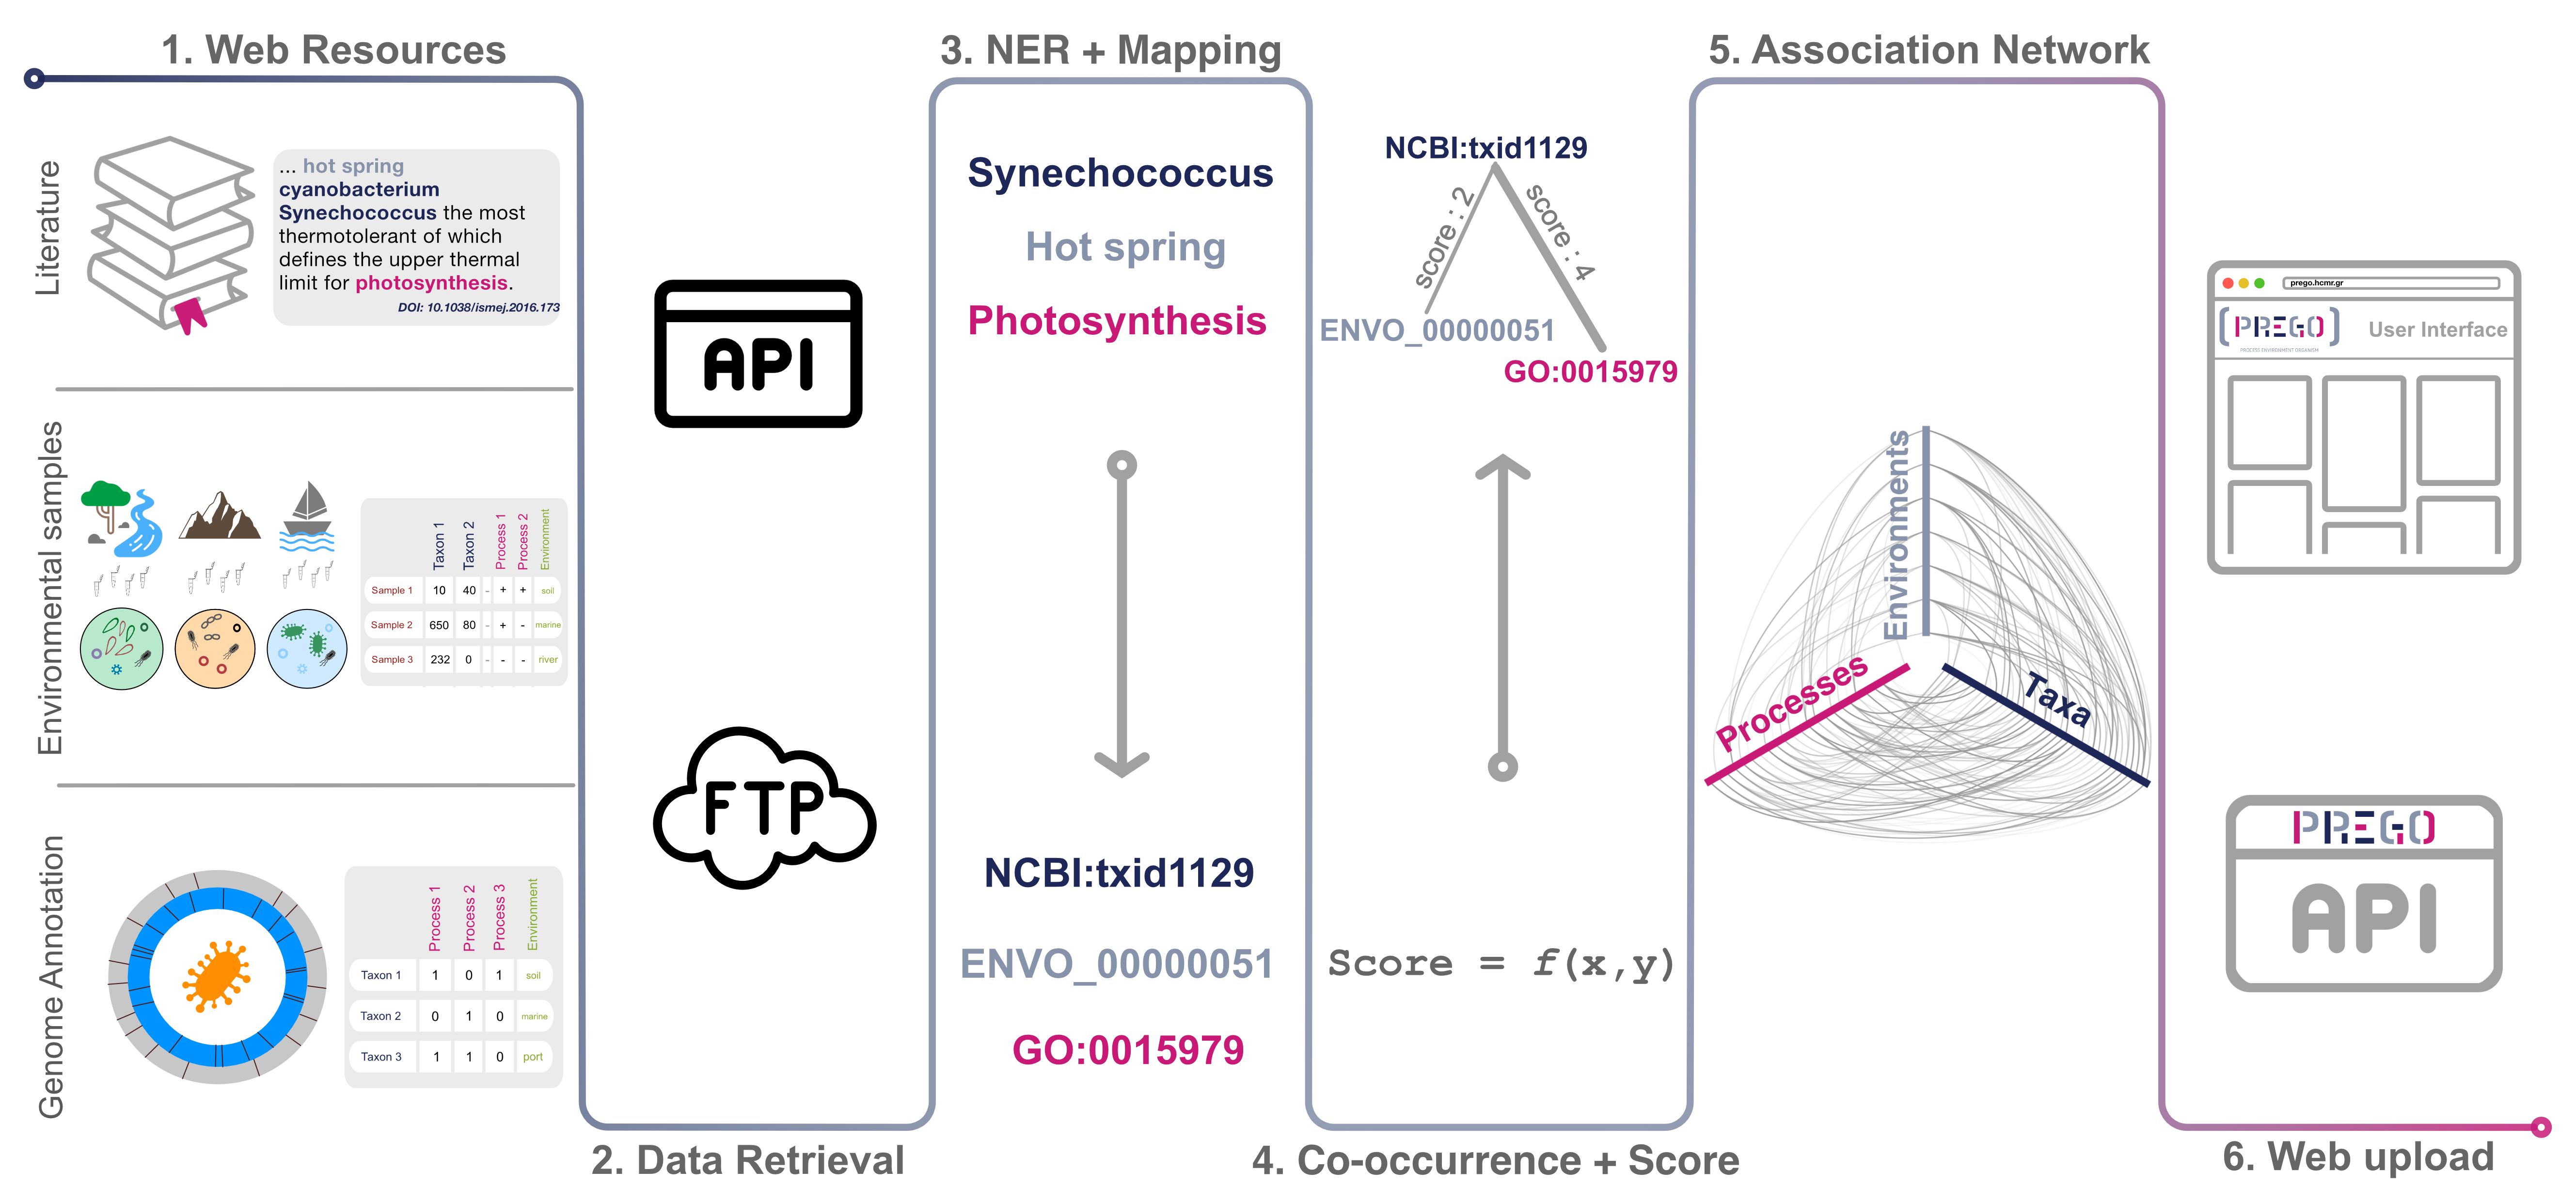
\includegraphics[width=0.98\columnwidth]{figures/prego_analysis_horizontal.png}
      \caption{
         PREGO analysis methodology. PREGO periodically retrieves three distinct types of data from open access resources. Scientific text, environmental sample data and genomic annotations are handled with respective methodologies in order to standardize their entities. Named Entity Recognition and Co-occurrence analysis is the common framework in order to build a weighted association network with nodes being the entity identifiers. Lastly, all these associations are available through a Web interface and an API. All these steps have been implemented in an autonomous way with regular cycles of updates (see Appendix B).
      }
   \end{figure}



% RPEGO RESULTS
\subsection{Results \& Validation}



\begin{figure}[h]
   \label{prego_ui}
   \centering
   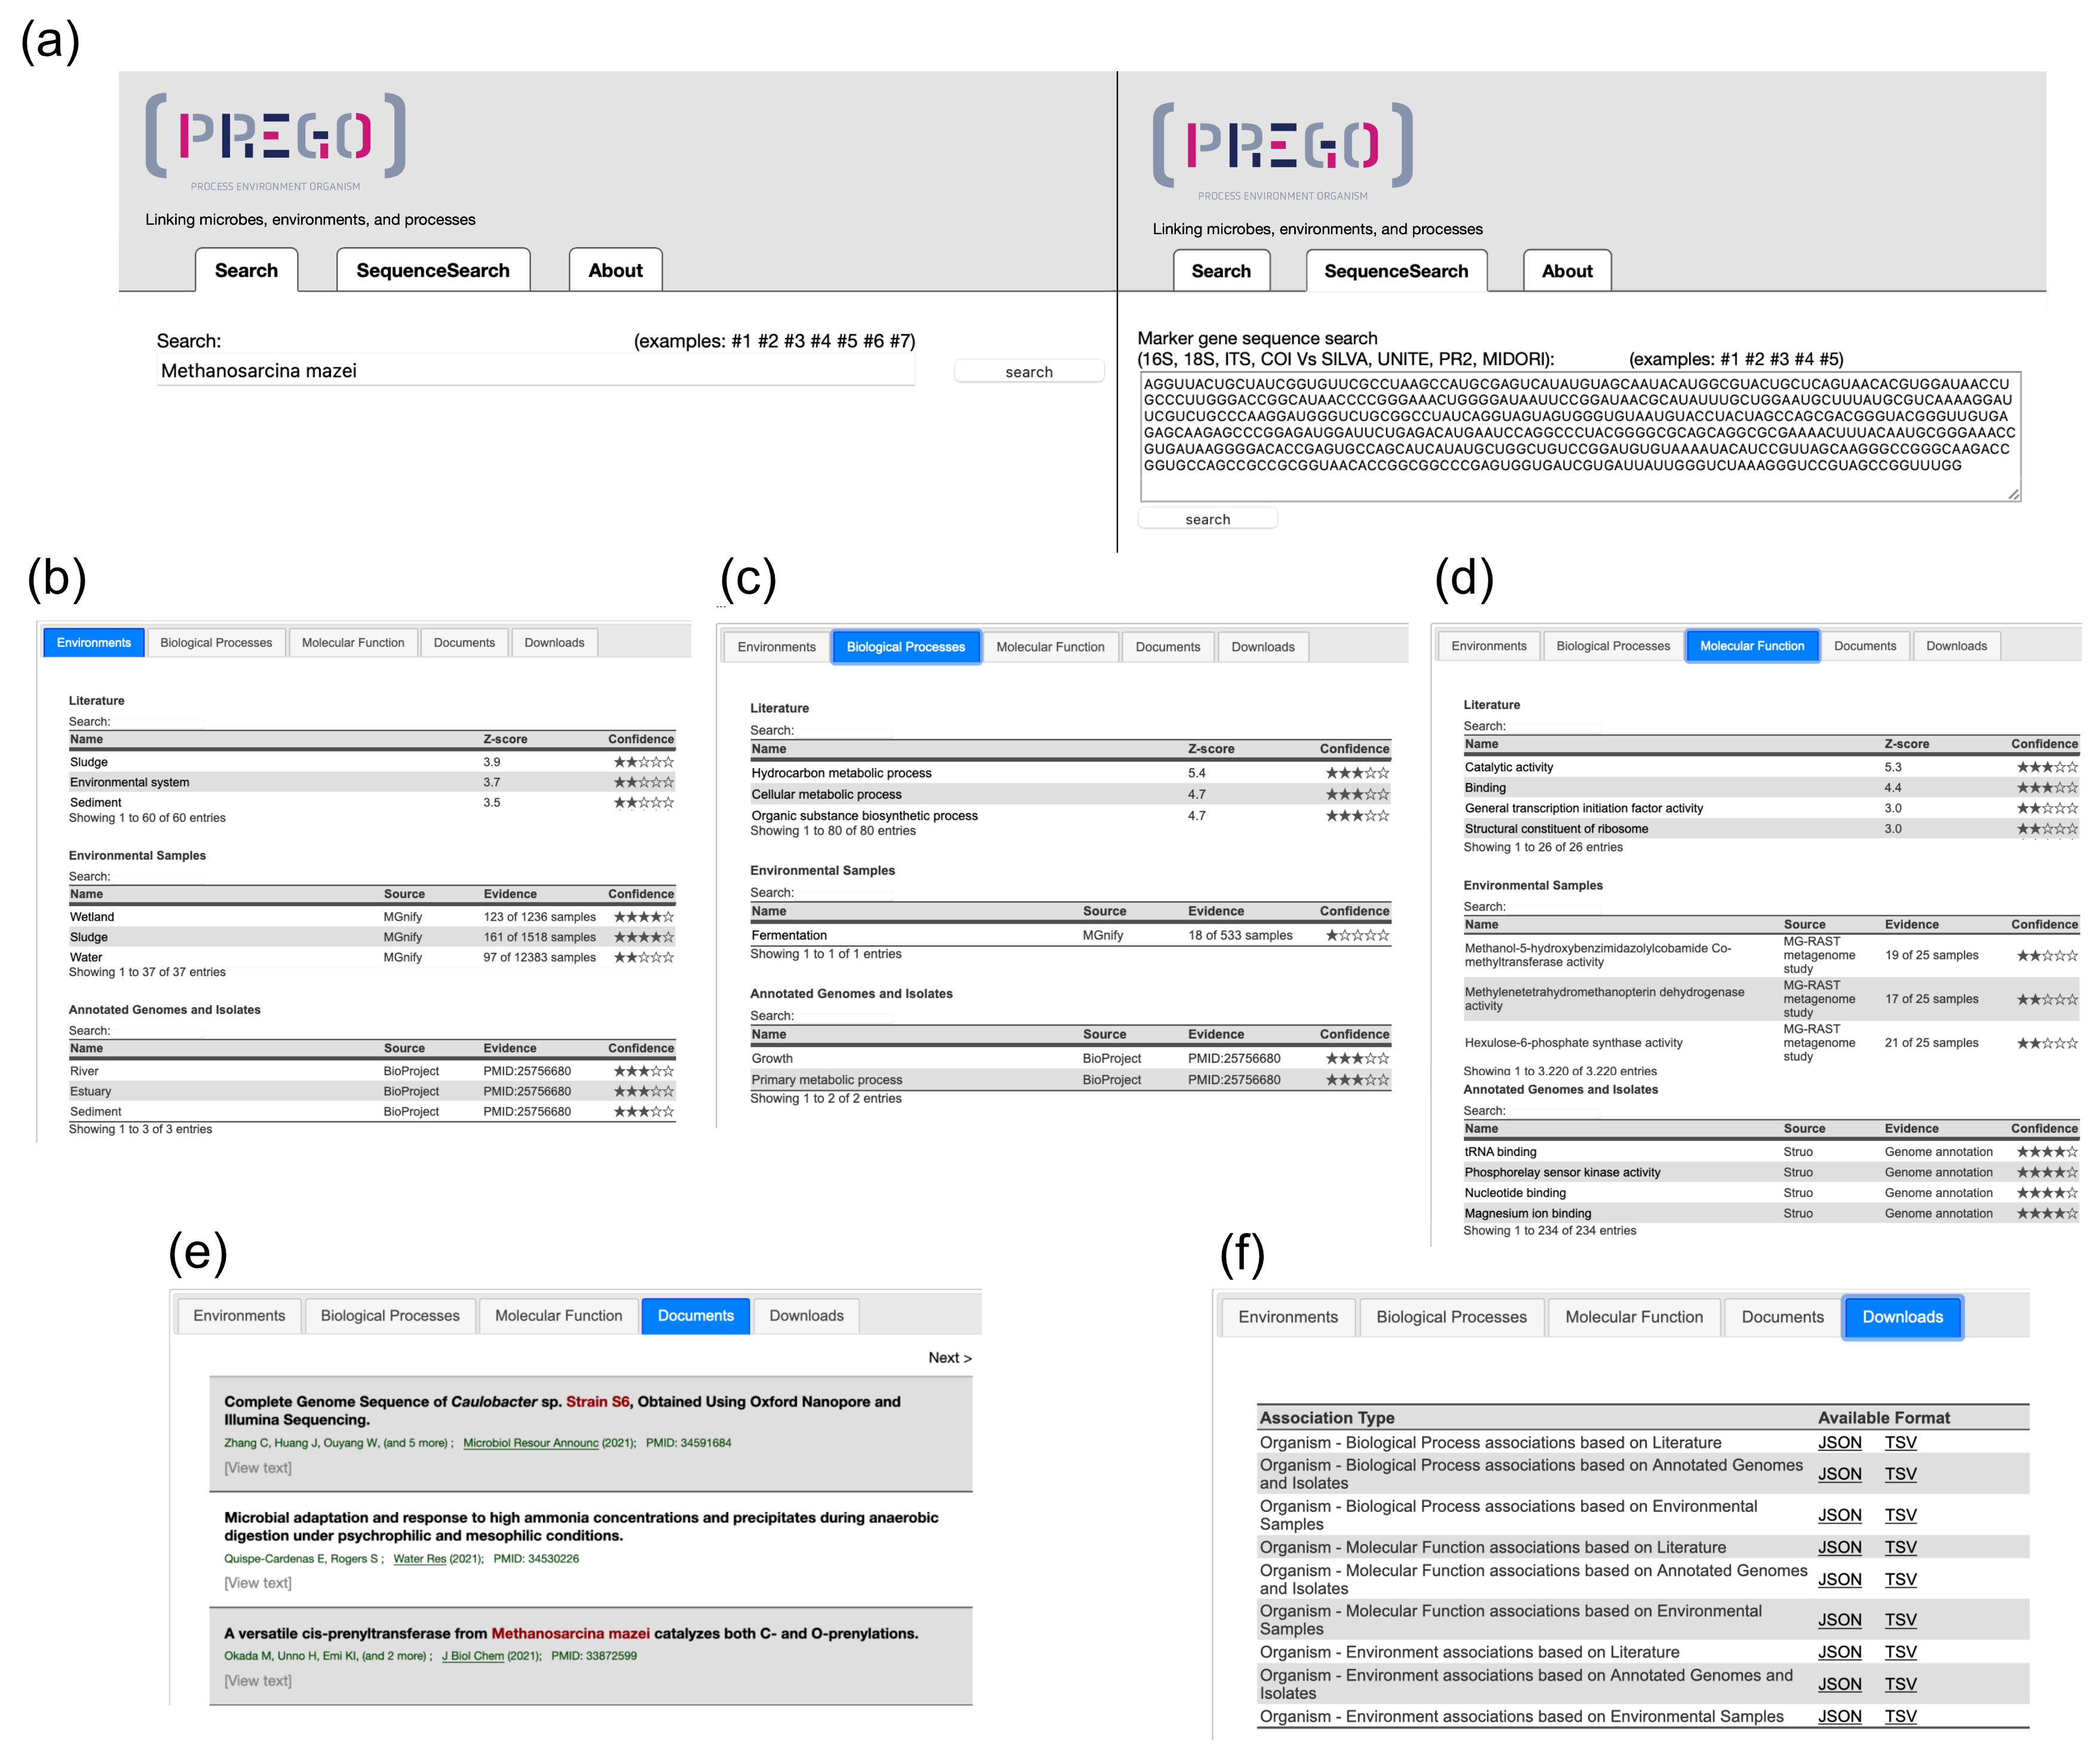
\includegraphics[width=0.98\columnwidth]{figures/prego_ui.png}
   \caption{
      PREGO web user interface. 
      (a) There are two search fields, plain text and taxa sequences. 
      (b-d) three associations tabs each one presenting associations of the querred entity with the respective entities, Environments (b), Biological Process (c ) and Molecular Function (d). 
      Three channels of information are distinguishing the associations based on the original data. 
      (e) Documents tab presents the scientific articles that mention the queried entity highlighted with color. 
      (f) Downloads tab provides the associations of each channel (when available) to be downloaded in JSON and TSV format.
   }
\end{figure}





\begin{figure}[h]
   \label{fig:prego_ui_resources}
   \centering
   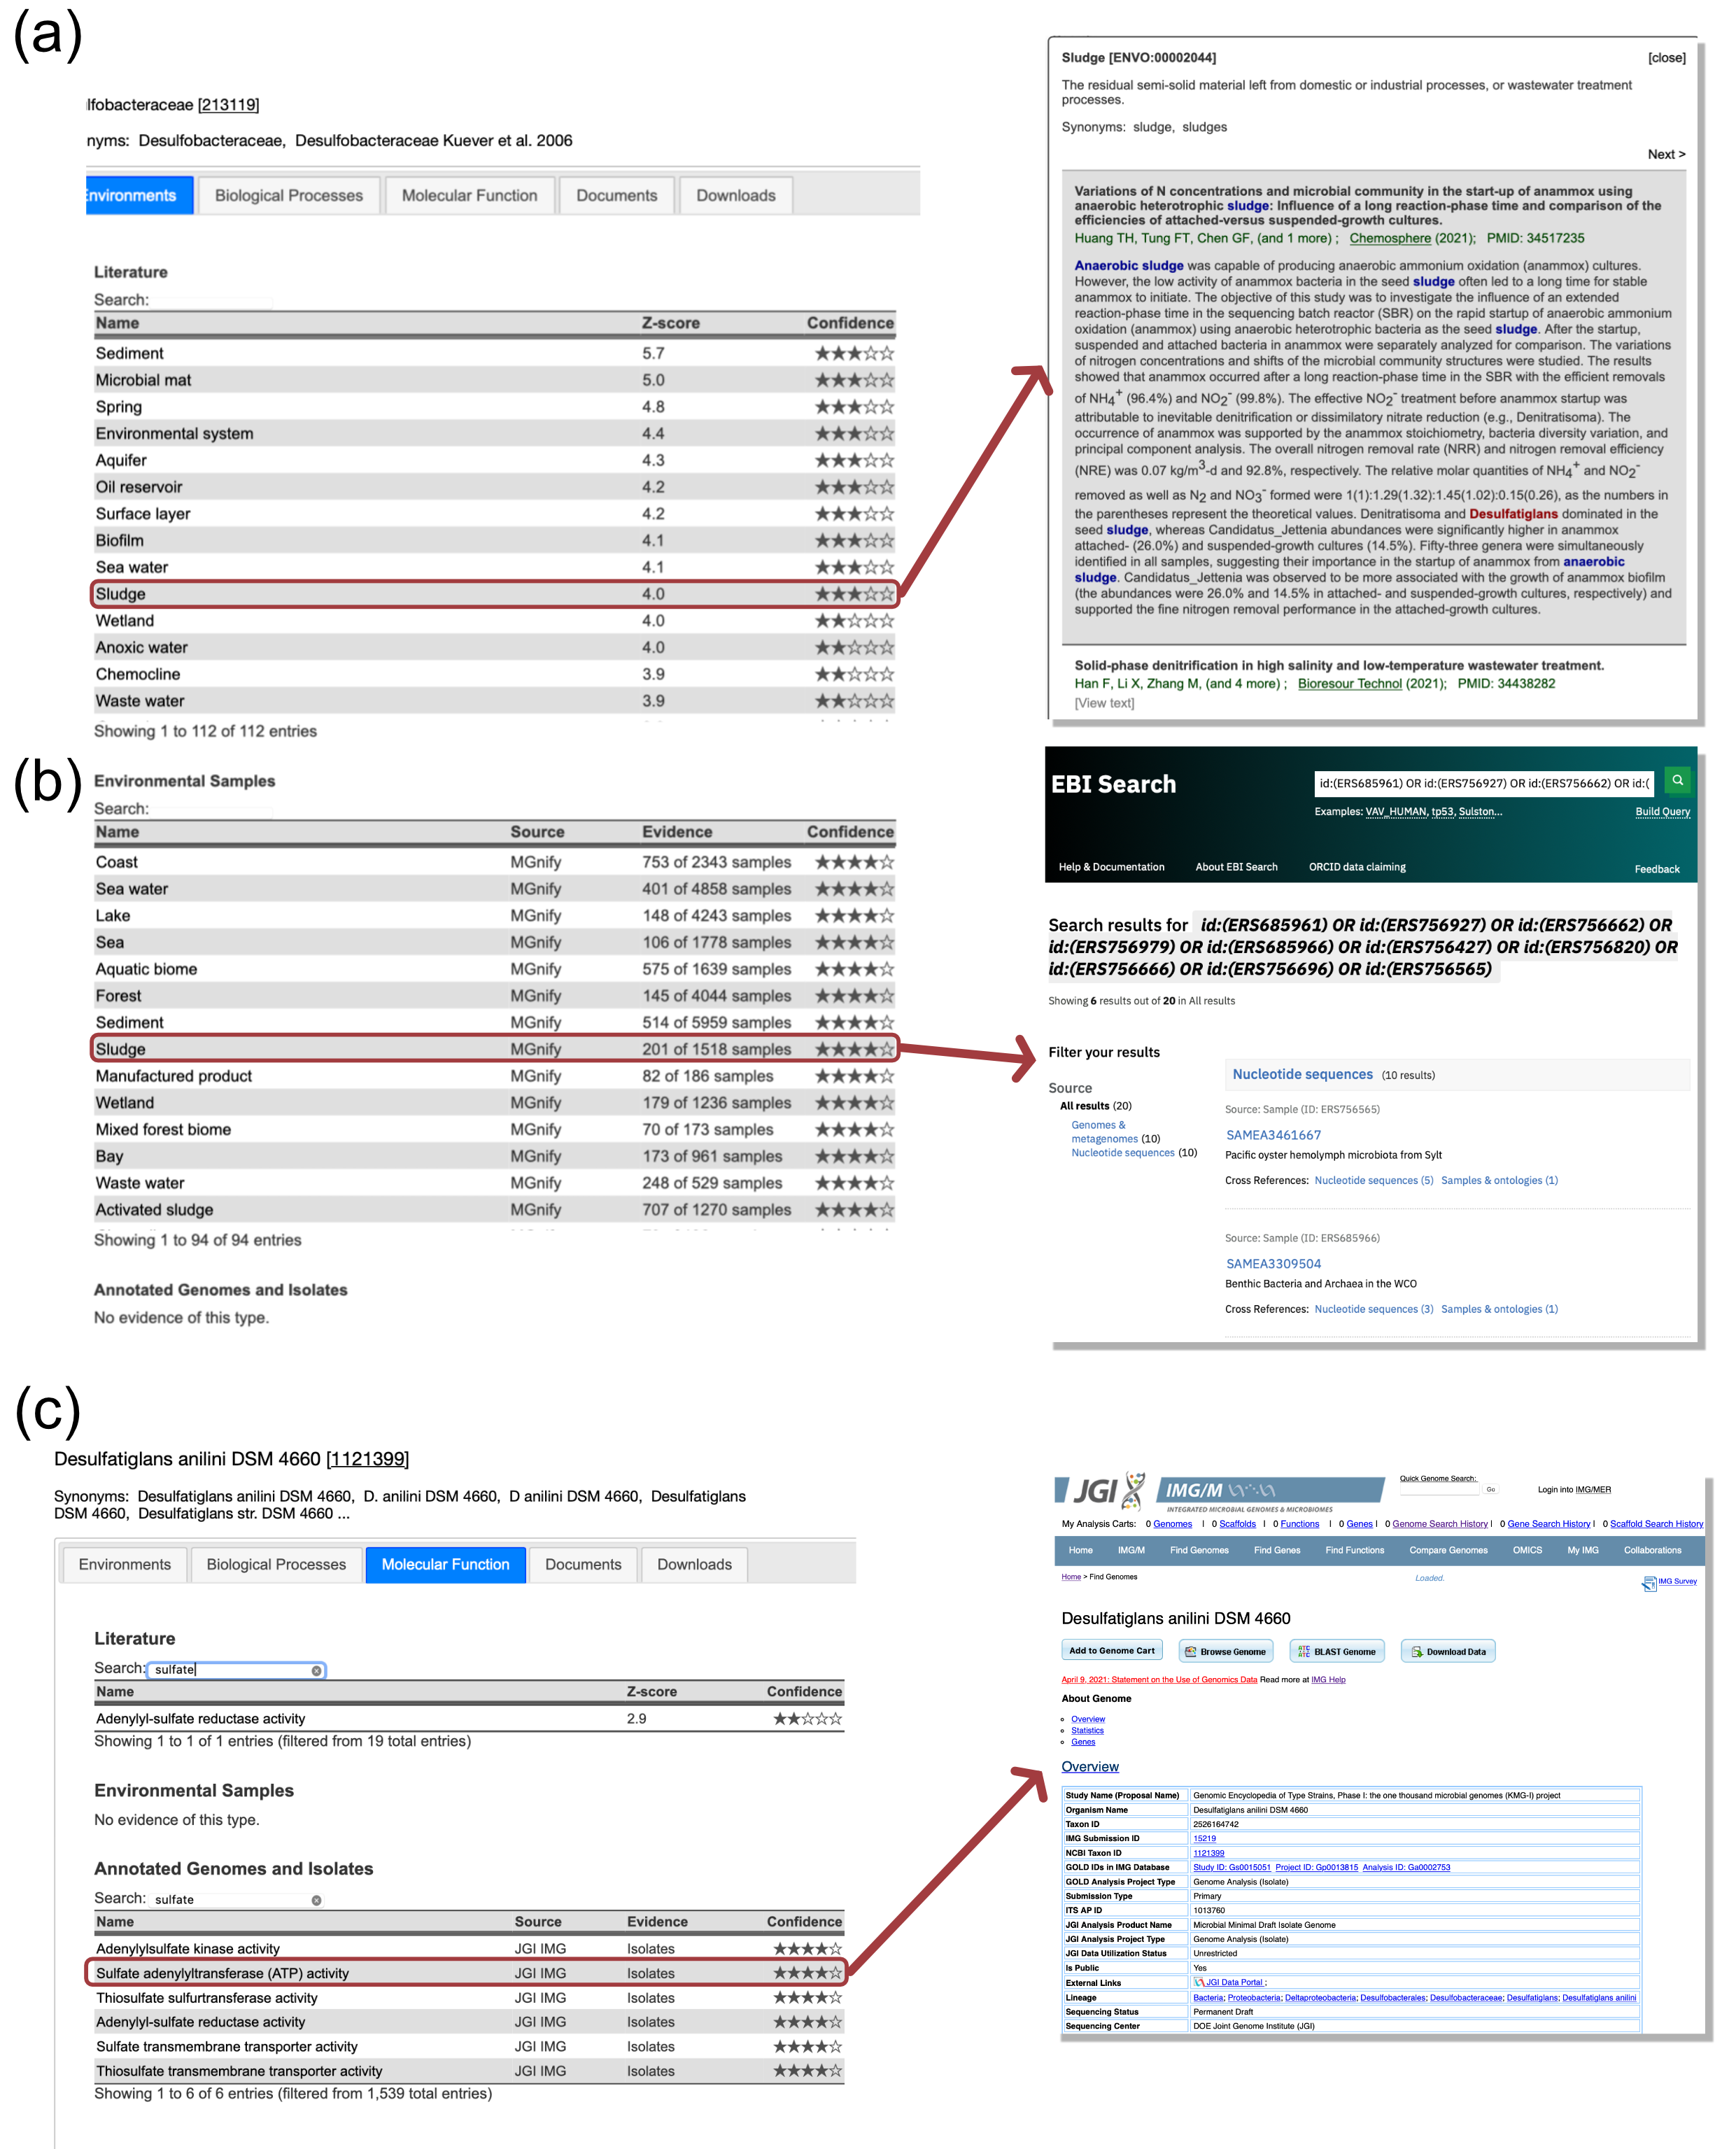
\includegraphics[width=0.98\columnwidth]{figures/prego_ui_resources.png}
   \caption{ 
      Each association is supported by original data. 
      (a) Literature channel has a pop-up functionality that displays the scientific articles that each specific association occurs with highlighted color. 
      (b) Environmental Samples channel redirects to the samples that support the specific association (currently only is supported MGnify). 
      (c) Annotated Genomes channel similarly redirects to the isolates ids that each association is based on (both Struo and JGI IMG are supported).
   }
\end{figure}



kljfdfg~\ref{fig:prego_ui_resources}





   \subsubsection*{PREGO contents}



   % SOURCE DATABASES TABLE
   \begin{table}[]
      \begin{tabular}{@{}ccccc@{}}
      \toprule
      \textbf{Source} & \textbf{\# items} & \textbf{Data type} & \textbf{Metadata} & \textbf{License} \\ \midrule
      \begin{tabular}[c]{@{}c@{}}MEDLINE and \\ PubMed\end{tabular} & 33 million & abstracts (text) & no & NLM Copyright \\
      \begin{tabular}[c]{@{}c@{}}PubMed Central \\ OA Subset\end{tabular} & 2.7 million & full article (text) & no & \begin{tabular}[c]{@{}c@{}}CC for Commercial, \\ non-commercial\end{tabular} \\
      JGI IMG & 9,644 & \begin{tabular}[c]{@{}c@{}}Isolates Annotated \\ genomes\end{tabular} & yes & JGI Data Policy \\
      Struo & 21,276 & Annotated genomes & no & MIT, CC BY-SA 4.0 \\
      BioProject & 18,752 & \begin{tabular}[c]{@{}c@{}}Annotated genomes \\ with abstracts (text)\end{tabular} & yes & INSDC policy \\
      \multirow{2}{*}{MG-RAST} & 16,096 & markergene samples & yes & CC0 \\
      & 7,965 & metagenomic samples & yes & CC0 \\
      MGnify & 10,500 & markergene samples & yes & CC-BY, CC0 \\ \bottomrule
      \end{tabular}
      
      \caption{
         Source databases that are integrated in PREGO and the number of items retrieved. 
         The Open Access subset of PubMed Central has Creative Commons licence available for commercial and noncommercial use. 
         JGI has its own licence, the same applies for BioProject, MEDLINE and PubMed as well.
      }
   \end{table}






   % PREGO ENTITIES AFTER NER AND MAPPING
   \begin{table}[]
      \begin{tabular}{@{}cccrccc@{}}
      \toprule
      \textbf{Channel} & \textbf{Source} & \multicolumn{2}{c}{\textbf{Taxonomy}} & \textbf{\begin{tabular}[c]{@{}c@{}}Environ- \\ ments\end{tabular}} & \textbf{\begin{tabular}[c]{@{}c@{}}Biological \\ Processes\end{tabular}} & \textbf{\begin{tabular}[c]{@{}c@{}}Molecular \\ Functions\end{tabular}} \\ \midrule
      \multirow{3}{*}{Literature} & \multirow{3}{*}{\begin{tabular}[c]{@{}c@{}}MEDLINE \\ PubMed - \\ PMC OA\end{tabular}} & Strains & 8,929 & \multirow{3}{*}{1,077} & \multirow{3}{*}{15,079} & \multirow{3}{*}{7,318} \\
      &  & Species & 240,377 &  &  &  \\
      &  & Total & 342,506 &  &  &  \\
      \multirow{9}{*}{\begin{tabular}[c]{@{}c@{}}Environ- \\ mental \\ samples\end{tabular}} & \multirow{3}{*}{\begin{tabular}[c]{@{}c@{}}MG-RAST \\ amplicon\end{tabular}} & Strains & 1,392 & \multirow{3}{*}{162} & \multirow{3}{*}{-} & \multirow{3}{*}{-} \\
      &  & Species & 4,324 &  &  &  \\
      &  & Total & 5,859 &  &  &  \\
      & \multirow{3}{*}{\begin{tabular}[c]{@{}c@{}}MG-RAST \\ metagenome\end{tabular}} & Strains & 2,522 & \multirow{3}{*}{258} & \multirow{3}{*}{-} & \multirow{3}{*}{3,839} \\
      &  & Species & 4,406 &  &  &  \\
      &  & Total & 7,157 &  &  &  \\
      & \multirow{3}{*}{\begin{tabular}[c]{@{}c@{}}MGnify \\ amplicon\end{tabular}} & Strains & 2 & \multirow{3}{*}{216} & \multirow{3}{*}{11} & \multicolumn{1}{l}{\multirow{3}{*}{-}} \\
      &  & Species & 1,471 &  &  & \multicolumn{1}{l}{} \\
      &  & Total & 2,955 &  &  & \multicolumn{1}{l}{} \\
      \multirow{9}{*}{\begin{tabular}[c]{@{}c@{}}Annotated\\Genomes \&\\Isolates\end{tabular}} & \multirow{3}{*}{JGI IMGisolates} & Strains & 2,398 & \multirow{3}{*}{241} & \multirow{3}{*}{-} & \multirow{3}{*}{3,670} \\
      &  & Species & 11,203 &  &  &  \\
      &  & Total & 13,849 &  &  &  \\
      & \multirow{3}{*}{STRUO} & Strains & 6 & \multirow{3}{*}{-} & \multirow{3}{*}{-} & \multirow{3}{*}{2,789} \\
      &  & Species & 19,289 &  &  &  \\
      &  & Total & 19,325 &  &  &  \\
      & \multirow{3}{*}{BioProject} & Strains & 5,754 & \multirow{3}{*}{309} & \multirow{3}{*}{626} & \multirow{3}{*}{-} \\
      &  & Species & 3,373 &  &  &  \\
      &  & Total & 9,393 &  &  &  \\
      \multirow{3}{*}{Total} & \multirow{3}{*}{All} & Strains & 12,840 & \multirow{3}{*}{1,090} & \multirow{3}{*}{15,091} & \multirow{3}{*}{7,971} \\
      &  & \multicolumn{1}{l}{} & \multicolumn{1}{l}{} &  &  &  \\
      &  & \multicolumn{1}{l}{} & \multicolumn{1}{l}{} &  &  &  \\ \bottomrule
      \end{tabular}

      \caption{
         The entities of PREGO after the NER and mapping of every source. 
         Counts of distinct entities of Taxa, Environments (ENVO terms), Biological Processes (Gene Ontology Biological process) and Molecular Function (Gene Ontology Molecular Function).
      }

   \end{table}







   % ASSOCIATIOS TABLE
   \begin{sidewaystable}
      \begin{tabular}{@{}cccccrcr@{}}
      \toprule
      \textbf{Channel} & \textbf{Source} & \textbf{\begin{tabular}[c]{@{}c@{}}Environments \\ - \\ Processes\end{tabular}} & \textbf{\begin{tabular}[c]{@{}c@{}}Environments \\ - \\ Functions\end{tabular}} & \textbf{Taxonomy} & \multicolumn{1}{c}{\textbf{\begin{tabular}[c]{@{}c@{}}Taxa \\ -\\  Environments\end{tabular}}} & \textbf{\begin{tabular}[c]{@{}c@{}}Taxa \\ - \\ Processes\end{tabular}} & \multicolumn{1}{c}{\textbf{\begin{tabular}[c]{@{}c@{}}Taxa \\ -\\ Function\end{tabular}}} \\ \midrule
      \multirow{3}{*}{Literature} & \multirow{3}{*}{\begin{tabular}[c]{@{}c@{}}MEDLINE \\ PubMed - \\ PMC OA\end{tabular}} & \multirow{3}{*}{883,997} & \multirow{3}{*}{422,579} & Strains & 69,968 & \multicolumn{1}{r}{590,630} & 384,079 \\
      &  &  &  & Species & 778,877 & \multicolumn{1}{r}{3,501,635} & 1,961,920 \\
      &  &  &  & Total & 1,669,608 & \multicolumn{1}{r}{7,969,310} & 4,613,827 \\
      \multirow{9}{*}{\begin{tabular}[c]{@{}c@{}}Environmental \\ samples\end{tabular}} & \multirow{3}{*}{\begin{tabular}[c]{@{}c@{}}MG-RAST \\ amplicon\end{tabular}} & \multirow{3}{*}{-} & \multirow{3}{*}{-} & Strains & 13,645 & \multirow{3}{*}{-} & \multicolumn{1}{c}{\multirow{3}{*}{-}} \\
      &  &  &  & Species & 39,007 &  & \multicolumn{1}{c}{} \\
      &  &  &  & Total & 53,439 &  & \multicolumn{1}{c}{} \\
      & \multirow{3}{*}{\begin{tabular}[c]{@{}c@{}}MG-RAST \\ metagenome\end{tabular}} & \multirow{3}{*}{-} & \multirow{3}{*}{620,846} & Strains & 262,106 & \multirow{3}{*}{-} & 8,626,328 \\
      &  &  &  & Species & 103,913 &  & 10,715,548 \\
      &  &  &  & Total & 372,301 &  & 19,950,096 \\
      & \multirow{3}{*}{\begin{tabular}[c]{@{}c@{}}MGnify \\ amplicon\end{tabular}} & \multirow{3}{*}{-} & \multirow{3}{*}{-} & Strains & 18 & - & \multicolumn{1}{l}{} \\
      &  &  &  & Species & 30,122 & \multicolumn{1}{r}{351} & \multicolumn{1}{c}{-} \\
      &  &  &  & Total & 111,976 & \multicolumn{1}{r}{2,097} & \multicolumn{1}{l}{} \\
      \multirow{9}{*}{\begin{tabular}[c]{@{}c@{}}Annotated Genomes \\ and Isolates\end{tabular}} & \multirow{3}{*}{\begin{tabular}[c]{@{}c@{}}JGI IMG\\ isolates\end{tabular}} & \multirow{3}{*}{-} & \multirow{3}{*}{-} & Strains & 8,229 & \multirow{3}{*}{-} & 3,461,693 \\
      &  &  &  & Species & 42,141 &  & 13,216,559 \\
      &  &  &  & Total & 50,888 &  & 16,821,850 \\
      & \multirow{3}{*}{STRUO} & \multirow{3}{*}{-} & \multirow{3}{*}{-} & Strains & \multicolumn{1}{c}{\multirow{3}{*}{-}} & \multirow{3}{*}{-} & 1,803 \\
      &  &  &  & Species & \multicolumn{1}{c}{} &  & 4,070,195 \\
      &  &  &  & Total & \multicolumn{1}{c}{} &  & 4,079,312 \\
      & \multirow{3}{*}{BioProject} & \multirow{3}{*}{-} & \multirow{3}{*}{-} & Strains & 3,263 & \multicolumn{1}{r}{7,473} & \multicolumn{1}{l}{} \\
      &  &  &  & Species & 4,187 & \multicolumn{1}{r}{4,294} & \multicolumn{1}{l}{} \\
      &  &  &  & Total & 7,641 & \multicolumn{1}{r}{12,169} & \multicolumn{1}{l}{} \\
      \multirow{3}{*}{Total} & \multirow{3}{*}{All} & \multirow{3}{*}{883,997} & \multirow{3}{*}{1,043,425} & Strains & 357,229 & \multicolumn{1}{r}{598,103} & 12,473,903 \\
      &  &  &  & Species & 998,247 & \multicolumn{1}{r}{3,506,280} & 29,964,222 \\
      &  &  &  & Total & 2,265,853 & \multicolumn{1}{r}{7,983,576} & 45,465,085 \\ \cmidrule(l){5-8} 
      \end{tabular}
   \end{sidewaystable}




% RPEGO DISCUSSION
\subsection{Discussion}


